\documentclass[a4paper,11pt]{tubsreprt}

\usepackage[utf8x]{inputenc}
\usepackage{xspace}
\usepackage{amsmath}
\usepackage{tabularx}
\usepackage{booktabs}
\usepackage{listings}
\lstset{basicstyle=\ttfamily}
\lstdefinestyle{cmd}{%
  frame=single,
  backgroundcolor=\color{tuGray20}
}
\lstdefinestyle{file}{%
  frame=single,
%   backgroundcolor=\color{tuGray20}
}
\usepackage[%
  colorlinks=true,
  linkcolor=tuRed100,
  citecolor=tuGreenDark]{hyperref}
\usepackage[ngerman]{babel}
\usepackage{caption, subcaption}
\usepackage{longtable}

\usepackage{enumerate,paralist}

\usepackage{tikz}

% glossaries
\usepackage[ngerman]{translator}
%Paket laden
\usepackage[
nonumberlist, %keine Seitenzahlen anzeigen
acronym,      %ein Abkürzungsverzeichnis erstellen
toc,          %Einträge im Inhaltsverzeichnis
section]      %im Inhaltsverzeichnis auf section-Ebene erscheinen
{glossaries}
\let\acs\gls
%Glossar-Befehle anschalten
\makeglossaries

% Kopiert von KOMA
\makeatletter
\providecommand\marg[1]{%
  {\ttfamily\char`\{}\meta{#1}{\ttfamily\char`\}}}
\providecommand\oarg[1]{%
  {\ttfamily[}\meta{#1}{\ttfamily]}}
\def\cmd#1{\cs{\expandafter\cmd@to@cs\string#1}}
\def\cmd@to@cs#1#2{\char\number`#2\relax}
\DeclareRobustCommand\cs[1]{\texttt{\char`\\#1}}

\newenvironment{Declaration}{%
%    \end{macrocode}
% \begin{macro}{\new@element}
%   Help macro to define new Declaration elements.
%    \begin{macrocode}
  \newcommand*{\new@element}[1]{%
    \expandafter\newcommand\expandafter*\csname X##1\endcsname{}%
    \expandafter\let\csname X##1\expandafter\endcsname
    \csname ##1\endcsname
    \expandafter\newcommand\expandafter*\csname new##1\endcsname[1]{%
%      \begingroup
%        \let\ensuremath\@firstofone
%        \let\textit\@firstofone
%        \lowercase{\def\@tempa{##1}}%
%        \pdfstringdef\@tempb{\label@base.\@tempa.####1}%
%        \xdef\@currentHref{\@tempb}%
%        \Hy@raisedlink{\hyper@anchorstart{\@currentHref}\hyper@anchorend}%
%        \label{desc:\label@base.\@tempa.####1}%
%      \endgroup
      \csname X##1\endcsname{####1}\ignorespaces
    }%
    \expandafter\let\csname ##1\expandafter\endcsname\csname new##1\endcsname
  }%
  \newcommand*{\new@xelement}[2]{%
    \expandafter\newcommand\expandafter*\csname X##1\endcsname{}%
    \expandafter\let\csname X##1\expandafter\endcsname
    \csname ##1\endcsname
    \expandafter\newcommand\expandafter*\csname new##1\endcsname[2]{%
%      \begingroup
%        \let\ensuremath\@firstofone
%        \let\textit\@firstofone
%        \lowercase{\def\@tempa{##1}}%
%        \pdfstringdef\@tempb{\label@base.\@tempa.####1.####2}%
%        \xdef\@currentHref{\@tempb}%
%        \Hy@raisedlink{\hyper@anchorstart{\@currentHref}\hyper@anchorend}%
%        \label{desc:\label@base.\@tempa.####1.####2}%
%      \endgroup
      \csname X##1\endcsname{####1}{##2{####2}}\ignorespaces
    }%
    \expandafter\let\csname ##1\expandafter\endcsname\csname new##1\endcsname
  }%
%    \end{macrocode}
%    \begin{macrocode}
  \new@element{Option}%
  \new@element{Macro}%
  \new@element{Environment}%
  \new@element{Counter}%
  \new@element{FloatStyle}%
  \new@element{PLength}%
  \new@element{Variable}%
  \new@xelement{OptionValue}{\PValue}%
%    \end{macrocode}
% \end{macro}
%    \begin{macrocode}
  \ifvmode\else\par\fi\addvspace{2\baselineskip}%
  \vspace{-\baselineskip}%
  \vspace{\z@ plus \baselineskip}%
  \noindent
  \start@Declaration
  \tabular{|l|}\hline\ignorespaces
}{%
  \\\hline\endtabular\nobreak\after@Declaration\nobreak\par\nobreak
  \vspace{1.5\baselineskip}\nobreak\vspace{-\baselineskip}\nobreak%
  \vspace{0pt minus .5\baselineskip}\nobreak%
  \aftergroup\@afterindentfalse\aftergroup\@afterheading
}
\newcommand*{\start@Declaration}{\hspace{-1em}}
\newcommand*{\after@Declaration}{}
% \begin{macro}{\Macro}
% \begin{macro}{\Option}
% \begin{macro}{\KOption}
% \begin{macro}{\OptionValue}
% \begin{macro}{\Environment}
% \begin{macro}{\Counter}
% \begin{macro}{\Length}
% \begin{macro}{\PLength}
% \begin{macro}{\FloatStyle}
% \begin{macro}{\Pagestyle}
% \begin{macro}{\Variable}
% \begin{macro}{\FontElement}
% \begin{macro}{\PName}
% \begin{macro}{\PValue}
% \begin{macro}{\Parameter}
% \begin{macro}{\OParameter}
% \begin{macro}{\AParameter}
% \begin{macro}{\PParameter}
% \begin{macro}{\POParameter}
%   \begin{description}
%   \item[\cs{Macro}] \LaTeX{} or \TeX{} macro
%   \item[\cs{Option}] class or package option
%   \item[\cs{KOption}] |\KOMAoptions| option
%   \item[\cs{Environment}] \LaTeX{} environment
%   \item[\cs{Counter}] \LaTeX{} counter
%   \item[\cs{Length}] \LaTeX{} length
%   \item[\cs{PLength}] \KOMAScript{} pseudo length
%   \item[\cs{Variable}] \KOMAScript{} variable
%   \item[\cs{FontElement}] \KOMAScript{} element that has its own font
%     selection
%   \item[\cs{PName}] name of a parameter of a macro or environment
%   \item[\cs{PValue}] value of a parameter of a macro or environment
%   \item[\cs{Parameter}] the mandatory parameter of a macro or environment
%   \item[\cs{OParameter}] the optional parameter of a macro or environment
%   \item[\cs{AParameter}] the alternativ parameter of a macro or environment
%   \item[\cs{PParameter}] the part-of-command parameter of a macro or
%     environment
%   \end{description}
%    \begin{macrocode}
\DeclareRobustCommand*{\Macro}[1]{\mbox{\texttt{\char`\\#1}}}
\DeclareRobustCommand*{\Option}[1]{\mbox{\texttt{#1}}}
\DeclareRobustCommand*{\KOption}[1]{\mbox{\Option{#1}\texttt=}}
\DeclareRobustCommand*{\OptionValue}[2]{\mbox{\texttt{#1=#2}}}
\DeclareRobustCommand*{\FloatStyle}[1]{\mbox{\texttt{#1}}}
\DeclareRobustCommand*{\Pagestyle}[1]{\mbox{\texttt{#1}}}
\DeclareRobustCommand*{\Environment}[1]{\mbox{\texttt{#1}}}
\DeclareRobustCommand*{\Counter}[1]{\mbox{\texttt{#1}}}
\DeclareRobustCommand*{\Length}[1]{\mbox{\texttt{\char`\\#1}}}
\DeclareRobustCommand*{\PLength}[1]{\mbox{\PValue{#1}}}
\DeclareRobustCommand*{\Variable}[1]{\mbox{\PValue{#1}}}
\DeclareRobustCommand*{\FontElement}[1]{\PValue{#1}}
\DeclareRobustCommand*{\PName}[1]{\texttt{\textit{#1}}}
\DeclareRobustCommand*{\PValue}[1]{\texttt{#1}}
\DeclareRobustCommand*{\Parameter}[1]{\texttt{\{}\PName{#1}\texttt{\}}}
\DeclareRobustCommand*{\OParameter}[1]{%
  \texttt{[%]
  }\PName{#1}\texttt{%[
    ]}}
\DeclareRobustCommand*{\AParameter}[1]{%
  \texttt{(%)
  }\PName{#1}\texttt{%(
    )}}
\DeclareRobustCommand*{\PParameter}[1]{\texttt{\{#1\}}}
\DeclareRobustCommand*{\POParameter}[1]{\texttt{[#1]}}
%    \end{macrocode}
% \end{macro}
% \end{macro}
% \end{macro}
% \end{macro}
% \end{macro}
% \end{macro}
% \end{macro}
% \end{macro}
% \end{macro}
% \end{macro}
% \end{macro}
% \end{macro}
% \end{macro}
% \end{macro}
% \end{macro}
% \end{macro}
% \end{macro}
% \end{macro}
% \end{macro}
% NOTE: taken from scrguide.cls

% \begin{environment}{desctable}
%   This is almost the same like \texttt{desctabular} but it uses a longtable
%   to allow page breaks.
%    \begin{macrocode}
\newenvironment{desctable}[1][2em]{%
  \onelinecaptionsfalse
  \start@desctab{#1}%
  \newcommand{\Endfirsthead}{\toprule\endfirsthead}%
  \newcommand{\Endhead}{\midrule\endhead}%
  \newcommand*{\standardfoot}{%
    \addlinespace[-.5\normalbaselineskip]\midrule
    \multicolumn{2}{r@{}}{\dots}\\
    \endfoot
    \addlinespace[-.5\normalbaselineskip]\bottomrule
    \endlastfoot
  }%
  \longtable{lp{\descwidth}}%
}{%
  \endlongtable
}
%    \end{macrocode}
% \end{environment}

% \begin{length}{\descwidth}
%   I need a length of local usage. I could have used |\@tempdima| or
%   another local length from kernel. But I've decided not to try to find a
%   unused length at \texttt{tabular} environment.
%    \begin{macrocode}
\newlength{\descwidth}
%    \end{macrocode}
% \end{length}

% \begin{macro}{\start@desctab}
%   This is the \emph{worker} macro of \texttt{desctable} and
%   \texttt{desctabular}. It does the complete calculations and definition of
%   the entry (something like |\item|) commands.
%    \begin{macrocode}
\newcommand*{\start@desctab}[1]{%
  \setlength{\descwidth}{\linewidth}%
  \addtolength{\descwidth}{-4\tabcolsep}%
  \addtolength{\descwidth}{-#1}%
  \setlength{\labelwidth}{\linewidth}%
  \addtolength{\labelwidth}{-2\tabcolsep}%
  \newcommand{\nentry}[2]{%
    \multicolumn{2}{p{\labelwidth}}{\raggedright##1}\\*%
    \hspace*{#1} & ##2\tabularnewline%
  }%
  \newcommand{\entry}[2]{\nentry{##1}{##2}[.5\baselineskip]}%
  \newcommand*{\pentry}[1]{%
    \entry{\PLength{##1}\IndexPLength[indexmain]{##1}}}%
  \newcommand*{\pventry}[1]{\entry{\PValue{##1}}}%
  \newcommand*{\mentry}[1]{\entry{\Macro{##1}}}%
  \newcommand*{\ventry}[1]{%
    \entry{\Variable{##1}%\IndexVariable[indexmain]{##1}%
    }%
  }%
  \newcommand*{\feentry}[1]{%
    \entry{\FontElement{##1}\IndexFontElement[indexmain]{##1}}%
  }%
  \newcommand*{\oentry}[1]{%
    \entry{\Option{##1}\IndexOption[indexmain]{##1}}%
  }%
}
% \end{macro}

\makeatother

% xspace für tubslatex-Logo
\makeatletter
\g@addto@macro{\tubslatex}{\xspace}
\makeatother

\def\example{\par\smallskip\noindent\textit{Beispiel: }}

% Schreibt 'Beispiel vor den folgenden Inhalt und rückt alles nach dem ersten
% Absatz um 2em ein.
\newenvironment{Example}{%
\begingroup
\leftskip2em
\par\smallskip\noindent\hspace*{-2em}\textit{Beispiel: }
}{%
\par\endgroup
}

% Umgebung: 'Wichtig:' ...
\newenvironment{important}{%
  \begin{description}
    \item[\itshape\mdseries\rmfamily Wichtig:]
}{%
  \end{description}
}

% Umgebung: 'Hinweis'
\newenvironment{hint}{%
  \begin{description}
    \item[\itshape\mdseries\rmfamily Hinweis:]
}{%
  \end{description}
}


\newcommand{\zB}{\mbox{z.\,B.}\xspace}

% Beamer-Macros
% Copyright 2003--2007 by Till Tantau
% Copyright 2010 by Vedran Mileti\'c
%
% This file may be distributed and/or modified
%
% 1. under the LaTeX Project Public License and/or
% 2. under the GNU Free Documentation License.
%
% See the file doc/licenses/LICENSE for more details.

% $Header: /home/vedranm/bitbucket/beamer/doc/beamerug-macros.tex,v 14743c450e2c 2010/06/17 09:25:56 rivanvx $

\def\beamer{\textsc{beamer}}
\def\pdf{\textsc{pdf}}
\def\pgfname{\textsc{pgf}}
\def\translatorname{\textsc{translator}}
\def\pstricks{\textsc{pstricks}}
\def\prosper{\textsc{prosper}}
\def\seminar{\textsc{seminar}}
\def\texpower{\textsc{texpower}}
\def\foils{\textsc{foils}}

{
  \makeatletter
  \global\let\myempty=\@empty
  \global\let\mygobble=\@gobble
  \catcode`\@=12
  \gdef\getridofats#1@#2\relax{%
    \def\getridtest{#2}%
    \ifx\getridtest\myempty%
      \expandafter\def\expandafter\strippedat\expandafter{\strippedat#1}
    \else%
      \expandafter\def\expandafter\strippedat\expandafter{\strippedat#1\protect\printanat}
      \getridofats#2\relax%
    \fi%
  }

  \gdef\removeats#1{%
    \let\strippedat\myempty%
    \edef\strippedtext{\stripcommand#1}%
    \expandafter\getridofats\strippedtext @\relax%
  }

  \gdef\stripcommand#1{\expandafter\@gobble\string#1}
}

\providecommand\href[2]{\texttt{#1}}

\def\printanat{\char`\@}

\def\declare#1{{\color{red!75!black}#1}}
%\def\declare{\afterassignment\translatormanualdeclare\let\next=}
%\def\translatormanualdeclare{\ifx\next\bgroup\bgroup\color{red!75!black}\else{\color{red!75!black}\next}\fi}

\def\command#1{\list{}{\leftmargin=2em\itemindent-\leftmargin\def\makelabel##1{\hss##1}}%
\item\extractcommand#1@\par\topsep=0pt}
\def\endcommand{\endlist}
\def\extractcommand#1#2@{\strut\declare{\texttt{\string#1}}#2%
  \index{\stripcommand#1@\protect\myprintocmmand{\stripcommand#1}}}

%\let\textoken=\command
%\let\endtextoken=\endcommand

\def\myprintocmmand#1{\texttt{\char`\\#1}}

\def\example{\par\smallskip\noindent\textit{Beispiel: }}
\def\themeauthor{\par\smallskip\noindent\textit{Theme author: }}

\def\environment#1{\list{}{\leftmargin=2em\itemindent-\leftmargin\def\makelabel##1{\hss##1}}%
\extractenvironement#1@\par\topsep=0pt}
\def\endenvironment{\endlist}
\def\extractenvironement#1#2@{%
\item{{\ttfamily\char`\\begin\char`\{\declare{#1}\char`\}}#2}%
  {\itemsep=0pt\parskip=0pt\item{\meta{environment contents}}%
  \item{\ttfamily\char`\\end\char`\{\declare{#1}\char`\}}}%
  \index{#1@\protect\texttt{#1} environment}%
  \index{Environments!#1@\protect\texttt{#1}}}

\def\classoption#1{\list{}{\leftmargin=2em\itemindent-\leftmargin\def\makelabel##1{\hss##1}}%
\item{{\ttfamily\char`\\documentclass[\declare{#1}]\char`\{beamer\char`\}}}
  \index{#1@\protect\texttt{#1} class option}%
  \index{Class options for \textsc{beamer}!#1@\protect\texttt{#1}}%
  \par\topsep=0pt}
\def\endclassoption{\endlist}


\newcommand\beameroption[2]{\list{}{\leftmargin=2em\itemindent-\leftmargin\def\makelabel##1{\hss##1}}%
\item{{\ttfamily\char`\\setbeameroption\char`\{\declare{#1}{\normalfont\opt{#2}}\char`\}}}
  \index{#1@\protect\texttt{#1} beamer option}%
  \index{Beamer options!#1@\protect\texttt{#1}}%
  \par\topsep=0pt}
\def\endbeameroption{\endlist}


\def\smallpackage{\vbox\bgroup\package}
\def\endsmallpackage{\egroup\endpackage}

\def\package#1{\list{}{\leftmargin=2em\itemindent-\leftmargin\def\makelabel##1{\hss##1}}%
\extracttheme#1@usepackage@package@Packages@\par\topsep=0pt}
\def\endpackage{\endlist}
%\def\extracttheme#1#2@{%
%\item{{{\ttfamily\char`\\usepackage}#2{\ttfamily\char`\{\declare{#1}\char`\}}}}}

\def\theme#1#2#3#4{\list{}{\leftmargin=2em\itemindent-\leftmargin\def\makelabel##1{\hss##1}}%
\extracttheme#2@#1@#3@#4@\par\topsep=0pt}
\def\endtheme{\endlist}
\def\extracttheme#1#2@#3@#4@#5@{%
\item{{{\ttfamily\char`\\#3}#2{\ttfamily\char`\{\declare{#1}\char`\}}}}%
  \index{#1@\protect\texttt{#1} #4}%
  \index{#5!#1@\protect\texttt{#1}}
}

\def\class#1{\list{}{\leftmargin=2em\itemindent-\leftmargin\def\makelabel##1{\hss##1}}%
\extractclass#1@\par\topsep=0pt}
\def\endclass{\endlist}
\def\extractclass#1#2@{%
\item{{{\ttfamily\char`\\documentclass}#2{\ttfamily\char`\{\declare{#1}\char`\}}}}%
  \index{#1@\protect\texttt{#1} class}%
  \index{Classes!#1@\protect\texttt{#1}}}

\def\typesetsol#1{\texttt{\def\_{\char`\_}#1}}

\def\solution#1{\list{}{\leftmargin=2em\itemindent-\leftmargin\def\makelabel##1{\hss##1}}%
\item \textbf{Solution Template }\declare{\typesetsol{#1}}\par\topsep=0pt%
  \index{#1@\protect\typesetsol{#1} solution}%
  \index{Solutions!#1@\protect\typesetsol{#1}}}
\def\endsolution{\endlist}

\def\template#1{\list{}{\leftmargin=2em\itemindent-\leftmargin\def\makelabel##1{\hss##1}}%
\item {\ttfamily\char`\\setbeamertemplate\char`\{\declare{#1}\char`\}}\oarg{options}\opt{\meta{args}}\par\topsep=0pt}
\def\endtemplate{\endlist}
\newenvironment{template*}[1]{\list{}{\leftmargin=2em\itemindent-\leftmargin\def\makelabel##1{\hss##1}}%
\item \leavevmode\llap{\color{blue}\vtop
    to0pt{\llap{\textsc{appear-\!}}\vskip-3pt\llap{\textsc{ance}}\vss}\ \ }{\ttfamily\char`\\setbeamertemplate\char`\{\declare{#1}\char`\}}\oarg{options}\opt{\meta{args}}\par\topsep=0pt}
{\endlist}

\newenvironment{element}[4]{\list{}{\leftmargin=2em\itemindent-\leftmargin\def\makelabel##1{\hss##1}}%
\item \textbf{\ifx#2\semiyes Parent Beamer-Template\else%
    Beamer\applier#2{-Template}\applier#3{\applier#2{/}-Color}\applier#4{\ifx#2\yes/\else\ifx#3\yes/\fi\fi
      -Font}\fi}
    {\ttfamily{\declare{#1}}}\par\topsep=0pt%
  \edef\parameters{%
    \ifx#2\semiyes parent template\else%
    \applier#2{template}\applier#3{\applier#2{/}color}\applier#4{\ifx#2\yes/\else\ifx#3\yes/\fi\fi font}\fi}
  \index{#1@\protect\texttt{#1} \parameters}%
  \applier#2{\index{Beamer templates!#1@\protect\texttt{#1}}}%
  \applier#3{\index{Beamer colors!#1@\protect\texttt{#1}}}%
  \applier#4{\index{Beamer fonts!#1@\protect\texttt{#1}}}%
}
{\endlist}

\def\applier#1#2{\ifx#1\yes#2\fi}

\def\templateoptions{\par
  The following template options are predefined:
  \begin{itemize}}
\def\endtemplateoptions{\end{itemize}}

\def\itemoption#1#2{\item {\texttt{[\declare{#1}]}}#2}

%\def\itemoption#1{\item \declare{\texttt{#1}}%
%  \indexoption{#1}%
%}

%\def\indexoption#1{%
%  \index{#1@\protect\texttt{#1} option}%
%  \index{Options!#1@\protect\texttt{#1}}%
%}

\def\yes{\hbox to .6cm{\ding{51}\hfil}}
\def\semiyes{\hbox to .6cm{(\ding{51})\hfil}}
\def\no{\hbox to .6cm{\ding{55}\hfil}}

\def\choosecol#1{}%\ifx#1\yes\color{green!50!black}\else\color{red!50!black}\fi}

\def\templatefontcolor#1#2#3#4{%
  \item\declare{\texttt{#1}}\hfill%
  {\choosecol#2Template #2} {\choosecol#3Color #3} {\choosecol#4Font #4}\par}

\def\fontparents#1{Font parents: \texttt{#1}\par}
\def\colorparents#1{Color parents: \texttt{#1}\par}
\def\colorfontparents#1{Color/font parents: \texttt{#1}\par}

\def\templateinserts{\begin{itemize}}
\def\endtemplateinserts{\end{itemize}}

\def\iteminsert#1{\item {\texttt{\declare{\string#1}}}%
  \index{Inserts!\stripcommand#1@\protect\myprintocmmand{\stripcommand#1}}}

\newcommand\opt[1]{{\color{black!50!green}#1}}
\newcommand\oarg[1]{\opt{{\ttfamily[}\meta{#1}{\ttfamily]}}}
\newcommand\ooarg[1]{{\ttfamily[}\meta{#1}{\ttfamily]}}
\newcommand\sarg[1]{\opt{{\ttfamily\char`\<}\meta{#1}{\ttfamily\char`\>}}}
\newcommand\ssarg[1]{{\ttfamily\char`\<}\meta{#1}{\ttfamily\char`\>}}

%\def\opt{\afterassignment\translatormanualopt\let\next=}
\def\translatormanualopt{\ifx\next\bgroup\bgroup\color{black!50!green}\else{\color{black!50!green}\next}\fi}

\providecommand{\LyX}{L\kern-.1667em\lower.25em\hbox{Y}\kern-.125emX\@}

\newcommand{\beamernote}{\par\smallskip\noindent\llap{\color{blue}\vtop to0pt{\llap{\textsc{presen-\!}}\vskip-3pt\llap{\textsc{tation}}\vss}\ \ }}
\newcommand{\articlenote}{\par\smallskip\noindent\llap{\color{blue}\textsc{article}\ \ }}
\newcommand{\lyxnote}{\par\smallskip\noindent\llap{\color{blue}\textsc{lyx}\ \ }}
\newcommand{\appearancenote}{\par\smallskip\noindent\appearancenotetext}

\def\appearancenotetext{\llap{\color{blue}\vtop
    to0pt{\llap{\textsc{appear-\!}}\vskip-3pt\llap{\textsc{ance}}\vss}\ \ }}

\newcommand{\templatenote}{\par\smallskip\noindent\llap{\color{blue}\textsc{template}\ \ }}
\newcommand{\colornote}{\par\smallskip\noindent\llap{\color{blue}\textsc{color}\ \ }}
\newcommand{\fontnote}{\par\smallskip\noindent\llap{\color{blue}\textsc{font}\ \ }}

\newcommand{\genericthemeexample}[2][]{%
  \smallskip\par\noindent
  \pgfimage[width=.45\textwidth,page=1]{beamerug#2}\qquad\pgfimage[width=.45\textwidth,page=2]{beamerug#2}
  \smallskip\par}
\newenvironment{themeexample}[2][]
{\begin{theme}{usetheme}{{#2}#1}{presentation theme}{Presentation themes}
    \example\genericthemeexample{theme#2}
  }
{\end{theme}}
\newenvironment{innerthemeexample}[2][]
{\begin{theme}{useinnertheme}{{#2}#1}{inner theme}{Inner themes}
    \example\genericthemeexample{innertheme#2}
  }
{\end{theme}}
\newenvironment{outerthemeexample}[2][]
{\begin{theme}{useoutertheme}{{#2}#1}{outer theme}{Outer themes}
    \example\genericthemeexample{outertheme#2}
  }
{\end{theme}}
\newenvironment{colorthemeexample}[2][]
{\begin{theme}{usecolortheme}{{#2}#1}{color theme}{Color themes}
    \example\genericthemeexample{colortheme#2}
  }
{\end{theme}}
\newenvironment{fontthemeexample}[2][]
{\begin{theme}{usefonttheme}{{#2}#1}{font theme}{Font themes}
    \example\genericthemeexample{fonttheme#2}
  }
{\end{theme}}
\newenvironment{fontthemeexample*}[2][]
{\begin{theme}{usefonttheme}{{#2}#1}{font theme}{Font themes}}
{\end{theme}}

\def\partname{Part}

\colorlet{examplefill}{yellow!80!black}
\definecolor{graphicbackground}{rgb}{0.96,0.96,0.8}
\definecolor{codebackground}{rgb}{0.8,0.8,1}

\newenvironment{translatormanualentry}{\list{}{\leftmargin=2em\itemindent-\leftmargin\def\makelabel##1{\hss##1}}}{\endlist}
\newcommand\translatormanualentryheadline[1]{\itemsep=0pt\parskip=0pt\item\strut#1\par\topsep=0pt}
\newcommand\translatormanualbody{\parskip3pt}


%\newenvironment{command}[1]{
%  \begin{translatormanualentry}
%    \extractcommand#1\@@
%    \translatormanualbody
%}
%{
%  \end{translatormanualentry}
%}

%\def\extractcommand#1#2\@@{%
%  \translatormanualentryheadline{\declare{\texttt{\string#1}}#2}%
%  \removeats{#1}%
%  \index{\strippedat @\protect\myprintocmmand{\strippedat}}}


\renewenvironment{environment}[1]{
  \begin{translatormanualentry}
    \extractenvironement#1\@@
    \translatormanualbody
}
{
  \end{translatormanualentry}
}

\def\extractenvironement#1#2\@@{%
  \translatormanualentryheadline{{\ttfamily\char`\\begin\char`\{\declare{#1}\char`\}}#2}%
  \translatormanualentryheadline{{\ttfamily\ \ }\meta{environment contents}}%
  \translatormanualentryheadline{{\ttfamily\char`\\end\char`\{\declare{#1}\char`\}}}%
  \index{#1@\protect\texttt{#1} environment}%
  \index{Environments!#1@\protect\texttt{#1}}}



%\newenvironment{package}[1]{
%  \begin{translatormanualentry}
%    \translatormanualentryheadline{{\ttfamily\char`\\usepackage\opt{[\meta{options}]}\char`\{\declare{#1}\char`\}}}
%    \index{#1@\protect\texttt{#1} package}%
%    \index{Packages and files!#1@\protect\texttt{#1}}%
%    \translatormanualbody
%}
%{
%  \end{translatormanualentry}
%}



\newenvironment{filedescription}[1]{
  \begin{translatormanualentry}
    \translatormanualentryheadline{File {\ttfamily\declare{#1}}}%
    \index{#1@\protect\texttt{#1} file}%
    \index{Packages and files!#1@\protect\texttt{#1}}%
    \translatormanualbody
}
{
  \end{translatormanualentry}
}


\newenvironment{packageoption}[1]{
  \begin{translatormanualentry}
    \translatormanualentryheadline{{\ttfamily\char`\\usepackage[\declare{#1}]\char`\{translator\char`\}}}
    \index{#1@\protect\texttt{#1} package option}%
    \index{Package options for \textsc{translator}!#1@\protect\texttt{#1}}%
    \translatormanualbody
}
{
  \end{translatormanualentry}
}

\makeatletter
\def\index@prologue{\section*{Index}\addcontentsline{toc}{section}{Index}
  This index only contains automatically generated entries, sorry. A good
  index should also contain carefully selected keywords.
  \bigskip
}
% \c@IndexColumns=2
%   \def\theindex{\@restonecoltrue
%     \columnseprule \z@  \columnsep 35\p@
%     \twocolumn[\index@prologue]%
%        \parindent -30pt
%        \columnsep 15pt
%        \parskip 0pt plus 1pt
%        \leftskip 30pt
%        \rightskip 0pt plus 2cm
%        \small
%        \def\@idxitem{\par}%
%     \let\item\@idxitem \ignorespaces}
%   \def\endtheindex{\onecolumn}
% \def\noindexing{\let\index=\@gobble}

\makeatother


% Bindet Grafik mit Rahmen ein
\newcommand{\examplegraphic}[2][]{%
  \fboxsep0mm\fbox{\includegraphics[#1]{#2}}
}



%opening
\title{Das CorporateDesign in \LaTeX}
\subtitle{Anleitung und Dokumentation}
\author{Enrico Jörns}
\publishers{Institut fuer Lorem Ipsum} % to logo?


\begin{document}

\maketitle
\pagestyle{scrheadings}
\tableofcontents


\newcommand{\newdocumentclass}[1]{\textcolor{tuRed}{\lstinline{#1}}}

\chapter{Schnellstart}

\paragraph{Dokumente}
Die schnellste Methode ein Dokument im Corporate Design zu erstellen ist
das Laden einer der zur Verfügung stehenden Dokumentenklassen.
Für die Erstellung von Textdokumenten sind dies \newdocumentclass{tubsartcl},
\newdocumentclass{tubsreprt} und \newdocumentclass{tubsbook}.

\paragraph{Poster}
Die Klasse \newdocumentclass{tubsposter} kann zum Erstellen von Postern verwendet werden.
% tubsflyer?

\paragraph{Papierformat}
Die zu verwendende Papierformat sollte dabei als optionales Argument mit
übergeben werden. Für ein Dokument in DIN A4 ist dies \texttt{a4paper}.
Zur Verfügung stehen alle Papierformate A0 bis A6.

Standardmäßig wird die Titelseite in Dokumenten einfach mit dem Logo und einer
roten Trennlinie zwischen Kommunikations- und Absenderbereich versehen.

\paragraph{Präsentationen}
Um Präsentation zu erstellen existiert ein Style für \LaTeX-Beamer.
Dieser wird einfach mit \lstinline!\usetheme{tubs}! geladen.


\chapter{Dokumente}

Einfache Textdokumente können mit den Klassen \newdocumentclass{tubsartcl},
\newdocumentclass{tubsreprt} und \newdocumentclass{tubsbook} erstellt werden.

% \section{Bindekorrektur und Marginalen}

Da Dokumente normalerweise gedruckt werden und ggf. auch gebunden, werden
sie standardmäßig mit einer kleinen Bindekorrektur gesetzt, sodass das
Logo beim Drucken oder Abheften nicht abgeschnitten wird.
Diese Bindekorrektur kann mittels der Paketoption \texttt{bcor} angepasst werden.
Mit \texttt{bcor=0mm} wird sie beispielsweise deaktiviert.



\section{Titelseite}

Titelseiten können bei \LaTeX\ generell auf zwei verschiedene Arten erstellt
werden; entweder mit Hilfe des Befehls \lstinline{\maketitle} oder mit
der Umgebung \lstinline{titlepage}. Beide Varianten werden von tubslatex
unterstützt und leicht modifiziert.

\begin{Declaration}
  \Macro{maketitle}\OParameter{style}
\end{Declaration}

Die einfache Verwendung von \lstinline{\maketitle} erzeugt eine Titelseite
mit dem TU-Logo und einer roten Trennlinie zwischen Absender- und
Kommunikationsbereich.

Mit Hilfe des optionalen Arguments \PName{style} kann die Darstellung
der Titelseite geändert werden, indem aus einer Reihe vordefinierter Styles
ausgewählt wird.\bigskip

Neben den standardmäßig definierten Elementen für Haupttitelseiten werden
in \tubslatex noch ein paar zusätzliche definiert.

\begin{Declaration}
  \Macro{logo}\Parameter{logo}\\
  \Macro{titlepicture}\Parameter{file}\\
  \Macro{titleabstract}\Parameter{text}
\end{Declaration}

\Macro{logo} dient zur Darstellung eines zusätzlichen Absenders als Schrift
oder Bild. Es wird in allen Stilen im Absenderbereich auf der dem
TU-Logo gegenüberliegenden Seite dargestellt.
Mit \Macro{titlepicture} kann eine Bilddatei angegeben werden, die bei
Verwendung eines entsprechenden Styles auf der Titelseite dargestellt werden.
\Macro{titeabstract} erlaubt die Darstellung eines kurzen zusammenfassenden
Textes auf der Titelseite, sofern der gewählte Stil dies unterstützt.

\begin{Declaration}
  \XMacro{begin}\PParameter{\Environment{titlepage}}\\
  \quad\dots\\
  \XMacro{end}\PParameter{titlepage}
\end{Declaration}

Mit der \Environment{titlepage}-Umgebung können, wie von den Standardklassen
gewohnt, Titelseiten definiert werden.
% TODO: \showtubslogo  etc.

\begin{Declaration}
  \XMacro{begin}\PParameter{\Environment{titlerow}}%
    \OParameter{options}%
    \Parameter{gaussheight}\\
  \quad\dots\\
  \XMacro{end}\PParameter{titlerow}
\end{Declaration}

Die Umgebung \Environment{titlerow} erlaubt es dabei, die Titelelemente im 
Gaußraster anzulegen. Der Parameter \PName{gaussheight} gibt dabei
die Höhe des jeweiligen Elements in Segmenten an. Die Position der Elemente
ergibt sich aus der Reihenfolge der Definition.
Mit dem optionalen Parameter \PName{options} können Einstellung wie die Hintergrundfarbe oder ein Hintergrundbild übergeben werden.

\subsection{Vordefiniert Titel-Styles}

Es sind 3 einfache Styles vordefiniert.

\begin{center}
  \fboxsep0mm
  \begin{minipage}[t]{0.33\textwidth}
    \centering\sffamily
    \fbox{%
      \includegraphics[width=0.95\textwidth]{examples/article1.pdf}}
    [default]
  \end{minipage}%
  \begin{minipage}[t]{0.33\textwidth}
    \centering\sffamily
    \fbox{%
      \includegraphics[width=0.95\textwidth]{examples/titlestyle_image.pdf}}
    [image]
  \end{minipage}%
  \begin{minipage}[t]{0.33\textwidth}
    \centering\sffamily
    \fbox{%
      \includegraphics[width=0.95\textwidth]{examples/titlestyle_imagetext.pdf}}
    [imagetext]
  \end{minipage}

\end{center}

\section{Kopf-/ Fußzeile}

Standardmäßig wird die Fußzeile komplett leer gelassen und die Kopfzeile
wird mit Seitennummer rechts und Kapitelname links gesetzt. Bei zweiseitigem
Layout gilt dies für die ungeraden Seiten, gerade Seiten werden entsprechend
mit Seitennummer links und Kapitelname rechts gesetzt.

\begin{Declaration}
  \Macro{ihead}\Parameter{innen}\\
  \Macro{ohead}\Parameter{außen}
\end{Declaration}

Bei Bedarf können die Kopfzeilen individuell angepasst werden.
Dies geschieht mit den Befehlen \Macro{ihead} und \Macro{ohead}, welche
auf den gleichnamigen Kommandos aus dem Koma-Skript aufbauen und für eine
korrekte vertikale Positionierung sorgen.

\begin{Declaration}
  \Macro{headsepline}
\end{Declaration}


Die standardmäßig gesetzten kurzen Linien am jeweils oberen äußeren Ende des
Kopfbereiches sind im Makro \Macro{headsepline} definiert.
Dies kann bei Bedarf überschrieben werden.


\section{Seitenlayout}

Eine Seite im Corporate Design unterteilt sich grundlegend in 2 Bereiche.
Der Absenderbereich und der Kommunikationsbereich. Der Absenderbereich wird zur
Darstellung des TU-Siegelbandlogos und des Logos eines speziellen Instituts
oder einer Abteilung verwendet. Im Textteil dient er teilweise als Bereich für
Inhalte einer Kopf-/Fußzeile.

Der Absenderbereich kann entweder am Anfang oder am Ende der Seite platziert
werden. Dies beeinflusst auch das Gaußraster, es beginnt jeweils mit dem
größten Segment am Absenderbereich.

\begin{Declaration}
  \Option{a0paper}\\
  \Option{a1paper}\\
  \Option{a2paper}\\
  \Option{a3paper}\\
  \Option{a4paper}\\
  \Option{a5paper}\\
  \Option{a6paper}
\end{Declaration}

Für die Auswahl des verwendeten Papierformats stehen alle DIN A-Größen von
0 bis 6 zur Verfügung. Standardeinstellung ist \Option{a4paper}.

\begin{Declaration}
  \Option{landscape}
\end{Declaration}

Schaltet das Dokument in Querformat-Darstellung.

\begin{minipage}{0.45\textwidth}\sffamily\centering
  {\fboxsep0mm\fbox{\includegraphics[width=\textwidth]{examples/article_landscape.pdf}}}\\
  Dokument im Querformat
\end{minipage}


\begin{important}
  Im Querformat hat das Gaußraster eine abweichende
  Segmentanzahl. Für alle gängigen Formate sind im Querformat \emph{6 Segmente}
  definiert. Daher lösen Layouts, die für hochformatige Dokumente
  geschrieben wurden, im Querformat einen Fehler aus.
\end{important}


\begin{Declaration}
  \KOption{sender}\PName{Position}
\end{Declaration}

Mit der Option \Option{sender} kann die Position des Absenderbereiches
festgelegt werden. Mit der Einstellung \OptionValue{sender}{top} wird
der Absenderbereich am oberen Seitenende dargestellt. Dies ist auch die
Standardeinstellung. Wählt man dagegen \OptionValue{sender}{bottom}, so
wird der Absenderbereich am unteren Ende der Seite platziert

\begin{important}
  Die Positionierung des Absenderbereichs beeinflusst die Orientierung des
  Gaußrasters. Das größte Segment wird dabei immer so gesetzt, dass es direkt
  an den Absenderbereich anschließt und alle folgende von absteigender Höhe sind.
\end{important}



\begin{Declaration}
  \KOption{bcor}\PName{Wert}
\end{Declaration}

Die Bindekorrektur beschreibt einen zusätzlichen Abstand des eigentlichen
Darstellungsbereichs vom inneren Formatrand. Die Bindekorrektur
ist bei Textdokumenten standardmäßig auf Rahmenbreite voreingestellt.

Sinnvoll ist eine Bindekorrektur selbstverständlich zum einen für Bindungen,
wo sie der Breite des durch die Bindung verdeckten Bereiches entsprechen sollte.
Zum anderen ist sie aber auch für den Druckvorgang sinnvoll, da normale Drucker
keinen randlosen Druck ermöglichen. Die Bindekorrektur verhindert so \zB ein 'Abschneiden' des Siegellogos.
Soll das Dokument ohne Bindekorrektur dargestellt werden, so ist dies
mit \OptionValue{bcor}{0mm} möglich.

\begin{Declaration}
  \Option{twoside}
\end{Declaration}

Für das Setzen von zweiseitige Dokumente ist die Option \Option{twoside}
vorgesehen. Mit ihr wird von einseitigem Layout auf zweiseitiges Layout
umgeschaltet, was bedeutet, dass die Innenseite eines Dokuments abwechselnd
auf der linken und rechten Seite definiert ist. Die hat unter anderem Einfluss
auf definierte Ränder (Bindungskorrektur, Marginale).


\begin{Declaration}
  \Option{marginleft}\\
  \Option{marginright}
\end{Declaration}

Das setzen einer Marginale wird durch die Befehle \PName{marginleft} und
\PName{marginright} vereinfacht. Diese setzen jeweils auf der linken (inneren)
bzw. rechten (äußeren) Seite des Dokumentes eine Marginale, deren Breite
einem Element im Spaltenraster entspricht.


\section{Schrift}

Dokumente im Corporate Design werden allgemein in der Schrift \emph{Nexus}
gesetzt.
Diese wird standardmäßig bei allen Dokumenten geladen. Auf eine explizite
Angabe der Schriftgröße in den Dokumentenoptionen sollte nach Möglichkeit
verzichtet werden, da für die jeweiligen Papierformate spezielle
Schriftgrößen vordefiniert sind und geladen werden.
Das Laden anderer Schriftgrößen führt im Vergleich dazu teilweise zu stark abweichenden Ergebnissen.

Für wichtige Standard-Elemente gibt es des weiteren vordefinierte Koma-Fonts.


\begin{desctable}
\entry{\PValue{headline}}{%
  Einfache Überschrift (groß)
}
\entry{\PValue{subheadline}}{%
  Unterüberschrift
}
\entry{\PValue{institute}}{%
  Institutsname im Logo-Bereich des Absenders.
}
% \entry{\PValue{infotext}}{%
% }
% \entry{\PValue{infotextitem}}{%
% }
\entry{\PValue{copytext}}{%
  Mengentext
}
\end{desctable}


\subsection{Farben}

Für eine Übersicht über die verfügbaren Farben siehe \ref{sec:colors}.%TODO...

\begin{Declaration}
  \Option{mono}
\end{Declaration}

Schwarz-Weiß-Darstellung der Standardelemente

\begin{Declaration}
  \Option{cmyk}
\end{Declaration}

CMYK-Darstellung der Standardelemente


% \noindent\hspace*{-\parindent}\fbox{\cmd{\maketitle}\oarg{asdf}\marg{asdf}}
\chapter{Plakate}

Plakate werden mit Hilfe der Klasse \newdocumentclass{tubsposter} erstellt.
Dabei kann Mittels der Option \texttt{style} zwischen der Darstellung als
normales Plakat oder als wissenschaftliches Plakat gewählt werden.

\section{Veranstaltungsplakate}

\begin{Declaration}
  \XMacro{begin}\PParameter{\Environment{tubsposter}}%
    \OParameter{options}\\
  \quad\dots\\
  \XMacro{end}\PParameter{tubsposter}
\end{Declaration}

Ein neues Plakat wird mit der Umgebung \Environment{tubsposter} erstellt.
Der optionale Parameter \PName{options} akzeptiert dabei die
unter \ref{} beschriebenen Optionen.

\begin{Declaration}
  \XMacro{begin}\PParameter{\Environment{posterrow}}%
    \OParameter{cols}\\%
  \quad\dots\\
  \XMacro{end}\PParameter{posterrow}%\\
%   \XMacro{begin}\PParameter{\Environment{posterrow*}}%
%     \OParameter{cols}\\%
%   \quad\dots\\
%   \XMacro{end}\PParameter{posterrow*}
\end{Declaration}

Einzelne Segmente im Gaußraster können mit der Umgebung \Environment{posterrow}
erzeugt werden.

\section{Wissenschaftliche Plakate}

\begin{Declaration}
  \XMacro{begin}\PParameter{\Environment{tubsposter}}%
    \OParameter{options}%
    \Parameter{rows}\\
  \quad\dots\\
  \XMacro{end}\PParameter{tubsposter}
\end{Declaration}

Für die Erstellung von wissenschaftlichen Plakaten wird ebenfalls die Umgebung
\Environment{tubsposter} verwendet, welche in diesem Fall jedoch einen
zusätzlichen Parameter \PName{rows} erwartet.
Damit wird die Anzahl an Modulzeilen bestimmt. Dies geschieht mittels
einer kommagetrennten Liste, wobei jedes Element entweder eine Länge
oder der Buchstabe 'X' sein kann. Eine Länge legt die Höhe der jeweiligen
Modulzeile genau fest, ein X sorgt dafür, dass alle mit X gekennzeichneten
Zeilen den restlichen zur Verfügung stehenden Platz gleichmäßig untereinander
aufteilen. Dieses Vorgehen ist an die Tabellen-Umgebung \Environment{tabularx}
angelehnt.

\begin{Example}
  \noindent\Macro{begin}\PParameter{\Environment{tubsposter}}
    \Parameter{3cm,X,5cm,X}\par
  \noindent Erzeugt 4 Modulzeilen, wobei die 1. 3cm und die 3. 5cm hoch sind.
  Die Zeilen 2 und 4 nehmen den Restlichen verfügbaren Platz ein
  und sind gleich hoch.
\end{Example}


\begin{Declaration}
  \XMacro{begin}\PParameter{\Environment{posterrow}}%
    \OParameter{cols}\\%
  \quad\dots\\
  \XMacro{end}\PParameter{posterrow}\\
  \XMacro{begin}\PParameter{\Environment{posterrow*}}%
    \OParameter{cols}\\%
  \quad\dots\\
  \XMacro{end}\PParameter{posterrow*}
\end{Declaration}

Die mit \Environment{tubsposter} angelegten Modulzeilen können nun jeweils mit
der Umgebung \Environment{posterrow} mit Inhalt gefüllt werden.
Dabei kann entweder direkt der gewünschte Inhalt geschrieben oder das optionale
Parameter \PName{cols} benutzt werden.
Dieses erlaubt die Definition zusätzlicher Spalten in der aktuellen Modulzeile.
Es wird wieder ein kommagetrennte Liste erwartet,
deren Elemente dieselbe Bedeutung haben wie bereits beschrieben, außer, dass
sie die Breite und nicht die Höhe definieren.

Der normale Abstand des Inhalts vom Rand der Modulbox beträgt halbe
Rahmenbreite. Für das Einfügen von Bildern etwa kann es sinnvoll sein,
diesen Rahmen wegzulassen. Dies geschieht mit der Sternchen-Variante
\Environment{posterrow*}.


\begin{Declaration}
  \XMacro{begin}\PParameter{\Environment{postercol}}%
    \OParameter{rows}\\%
  \quad\dots\\
  \XMacro{end}\PParameter{postercol}\\
  \XMacro{begin}\PParameter{\Environment{postercol*}}%
    \OParameter{rows}\\%
  \quad\dots\\
  \XMacro{end}\PParameter{postercol*}
\end{Declaration}

Die mit \Environment{posterrow} angelegten Spalten können jeweils mit 
\Environment{postercol} mit Inhalt gefüllt oder in neue Unterzeilen aufgeteilt 
werden.

\begin{Declaration}
  \XMacro{begin}\PParameter{\Environment{postersubrow}}\\%
  \quad\dots\\
  \XMacro{end}\PParameter{postersubrow}\\
  \XMacro{begin}\PParameter{\Environment{postersubrow*}}\\%
  \quad\dots\\
  \XMacro{end}\PParameter{postersubrow*}
\end{Declaration}

Die mit \Environment{postercol} angelegten Unterzeilen können jeweils mit 
\Environment{postercol} mit Inhalt gefüllt werden.

\begin{Example}

\end{Example}

\section{Seitenlayout}

% margin
% bcor
% sender=top/bottom


\section{Format}

\section{Farben}

\section{Befehle}

\section{Optionen}


\chapter{Briefe}

\chapter{Präsentationen}

% \section{Anwendung und Folienaufbau}

Grundsätzlich handelt es sich bei der Vorlage für Präsentationen lediglich um
ein \emph{theme} für das \emph{beamer}-Paket.
Für allgemeine Fragen zur Präsentationserstellung wir daher auf die
entsprechende Dokumentation\cite{beamer} verwiesen.

Beschrieben werden hier alle Besonderheiten des Corporate-Design-Themes.
Außerdem sollen einige damit verbundene allgemeine Hinweise gegeben werden.

Die Vorlage wird mit dem Beamer-Befehl \lstinline!\usetheme{tubs}! geladen.

\section{Titelfolie}

Die Titelfolie ist im Absender-/Kommunikations-Bereich-Layout mit
\gls{glos:siegelbandlogo} im Sinne der allgemeinen Gestaltungsprinzipien des
Corporate Design gehaltens.

Die Kommunikationsfläche ist nach Vorlage des \gls{glos:gaussraster}s
in drei Bereiche aufgeteilt:
Ein \emph{Bildbereich}, der ein Foto oder eine Grafik als Blickfang enthalten
sollte, darunter der \emph{Titelbereich}, der Präsentationstitel,
sowie alle relevanten Informationen trägt
und zum Abschluss ein einfarbiger (roter) Streifen.

Zusätzlich kann in der rechten oberen Ecke des Absenderbereichs ein
Instituts-Logo platziert werden.

\begin{minipage}{0.5\textwidth}
\begin{verbatim}
\title{Corporate Design}
\subtitle{Jetzt mit \LaTeX}
\author{Max Mustermann}

\begin{frame}[plain]
\titlepage
\end{frame}
\end{verbatim}
\end{minipage}
\fboxsep0mm
\begin{minipage}{0.5\textwidth}
\fbox{\includegraphics[width=0.9\textwidth]{examples/titelseite.pdf}}
\end{minipage}

\paragraph{Standardbefehle}

Es können die Standardbefehle zur Titelseitenerstellung, wie
\lstinline{\title},
\lstinline{\subtitle},
\lstinline{\author},
\lstinline{\titlegraphic}
und \lstinline{\logo} verwendet werden.

Die Titelseite wird normal mit \lstinline{\titlepage} erzeugt:

\begin{lstlisting}
\begin{frame}[plain]
  \titlepage
\end{frame}
\end{lstlisting}

\emph{Wichtig:} Der \lstinline{frame}-Umgebung muss die Option
\lstinline{[plain]} übergeben werden,
sonst kommt es zu einer falschen Darstellung!

\begin{Declaration}
  \Option{colorfoot}
\end{Declaration}

Mit der Beamer-Option \Option{colorfoot} wird die untere einfarbige Linie
der Titelseite statt in rot in der Farbe des benutzten Sekundärfarbklangs
dargestellt. Weitere Informationen zur Farbanpassung liefert
Kapitel~\ref{beamer:sec:color}


\subsection{Titelgrafik}

\begin{Declaration}
  \Macro{titlegraphic}\Parameter{Inhalt}
\end{Declaration}

\begin{sloppypar}
Dieser von \LaTeX-beamer bereitgestellte Befehl erlaubt in \tubslatex
die Darstellung von Inhalten im Bildbereich der Titel-Folie.
Der \PName{Inhalt} kann dabei ein beliebiges \LaTeX-Konstrukt sein
und wird am unteren Rande des Bildbereiches ausgerichtet dargestellt.

Im Normalfall wird als Titelgrafik allerdings eine Bild-Datei mittels
\lstinline{\includegraphics} eingebunden werden.
Diese kann (im Rahmen der allgemeinen Corporate Design-Richtlinien)% TODO:cite?
frei gewählt werden.
Das eingebundene Bild wird dabei automatisch randlos
auf den Darstellungsbereich skaliert und zugeschnitten, sofern keine
Standard-Optionen an \lstinline{\includegraphics} übergeben werden oder
manuell eine andere Einpassungsart gewählt wurde.

Innerhalb von \lstinline!\titlegraphic{}! stehen folgende
Optionen zur Einpassung des Bildes zur Verfügung:
\end{sloppypar}

%TODO: float-table + Link?
\begin{desctable}
\toprule
\entry{\PValue{clipped}}{%
  Automatisches Abschneiden. Dies ist die \emph{Standardeinstellung}.
  Das Bild wird dabei optimal in den Darstellungsbereich eingepasst
  (automatische Wahl von \PValue{hclip}/\PValue{vclip}).
}
\entry{\PValue{hclip}}{%
  Das Bild wird vertikal auf Höhe des Bildbereiches skaliert und (falls nötig)
  horizontal zugeschnitten.
}
\entry{\PValue{vclip}}{%
  Das Bild wird horizontal auf Breite des Bildbereiches skaliert und (falls nötig)
  vertikal zugeschnitten.
}
\entry{\PValue{scaled}}{%
  Horizontale \emph{und} vertikale Skalierung. Das Seitenverhältnis des
  Bildes kann dabei verändert und das Bild somit verzerrt werden.
}
\entry{\PValue{keepsize}}{%
  Es wird keinerlei Skalierung oder Beschneidung durchgeführt.
}
\bottomrule
\caption{Mögliche Parameter für \Macro{titlegraphic} zur
automatische Einpassung von Titelgrafik}
\end{desctable}

\begin{Example}
  \begin{lstlisting}
\titlegraphic[scaled]{\includegraphics{myimage.jpg}}
  \end{lstlisting}
  Fügt \textit{myimage.jpg} passend in den Bildbereich ein, indem es das Bild
  horizontal und vertikal skaliert.
\end{Example}

Im Prinzip ist das Seitenverhältnis des Quellbildes durch die automatische
Einpassung nicht besonders kritisch. Jedoch wird durch ein korrektes Verhältnis
sicher gestellt, dass keine wichtigen Teile des Bildes abgeschnitten werden.
In Tabelle \ref{tab:picratio} sind daher Bild-Seiten\-verhältnisse für
verschiedene Seitenverhältnisse der Präsentation aufgeführt.

\begin{table}[ht]
\centering
\begin{tabular}{ll}
\toprule
\bfseries Präsentation  & \bfseries  Bild  \\
\midrule
$3:4$   & $1:3{,}15$ \\
% Seitenverhältnis für 5:4 einfügen
$16:9$  & $1:4{,}30$ \\
$16:10$ & $1:3{,}83$ \\
\bottomrule
\end{tabular}
\caption{Bild-Seitenverhältnisse}
\label{tab:picratio}
\end{table}



\paragraph{Standardgrafik}

Zu Testzwecken oder falls kein eigenes Bild zur Hand ist,
kann alternativ ein Standardbild eingefügt werden, das die Front
des TU-Altgebäudes zeigt und gut mit den Standard-Folienfarben harmoniert.

Das Einfügen des Standardbildes ist mit dem Befehl
\linebreak\lstinline{\tuDefaultTitlegraphic} möglich,
der \lstinline!\titlegraphic{}! direkt als Argument übergeben werden kann.

\begin{example}
\begin{lstlisting}
\titlegraphic{\tuDefaultTitlegraphic}
\end{lstlisting}
\end{example}


\paragraph{Manuelle Einpassung}\hfill

\begin{Declaration}
  \Macro{titlegraphicswidth}\\
  \Macro{titlegraphicsheight}
\end{Declaration}

Zur manuellen Einpassung oder für das Erstellen von Grafiken mittels
\LaTeX-Befehlen ist die Dimension des Titelgrafik-Bereichs (Bildbereich) in den
beiden Längen \lstinline{titlegraphicswidth} und \lstinline{titlegraphicsheight}
hinterlegt.

% Das Titelbild wird generell an der unteren Kante des dafür vorgesehenen Bereichs ausgerichtet, sodass in falschem Seitenverhältnis vorliegene Bilder nach Oben 'rausgeschoben' werden.

\subsection{Logo}

Neben dem immer vorhandenen Siegelband-Logo der TU kann noch ein sekundäres Logo
dargestellt werden, welches das jeweilige Institut bzw. die jeweilige Abteilung
repräsentiert.

\begin{Declaration}
  \Macro{logo}\Parameter{Bild}
\end{Declaration}

Das mittels \lstinline{\logo} eingebundene Logo wird in der rechten oberen
Ecke des Absenderbereichs angezeigt und standardmäßig auch auf allen weiteren
Folien im Fußbereich, sofern nicht die Option \Option{nologoinfoot}
verwendet wird.

Das eingebundene Logo wird bei Verwendung von \Macro{includegraphics}
automatisch korrekt vertikal skaliert,
sofern keine manuelle Skalierung als Option angegeben wird.

% Die Verwendung von \lstinline{\logoheight} als Höhenbeschränkung für Grafiken
% stellt deren automatische korrekte vertikale Skalierung sicher.
% Das Seitenverhältnis der verwendeten Grafik-Datei ist dabei relativ
% frei, sollte jedoch nach Möglichkeit und Gründen der Lesbarkeit breiter sein als
% hoch.

\begin{example}
\begin{lstlisting}
\logo{
\includegraphics{institut.jpg}}
\end{lstlisting}
\end{example}

\begin{Declaration}
  \Macro{logoheight}
\end{Declaration}

Für allgemeine Inhalte kann auf die Höhe des Logo-Bereichs über die Länge
\Macro{logoheight} zugegriffen werden.

\section{Inhaltsfolien}

Das Layout der Inhaltsfolien ist relativ schlicht und bietet viel Platz.
Es zeichnet sich durch einen Kopfbereich, der Folientitle und evtl. eine
Inhaltsübersicht enthält, und einen Fußbereich, der neben Siegelband- und
Institutslogo allgemeine Informationen zur Präsentation liefert.
Auf den genaueren Aufbau des Kopfbereichs geht Kapitel~\ref{subsec:head},
auf den des Fußbereichs Kapitel~\ref{subsec:foot} ein.
% Die Überschrift ist im Kopfbereich grau hinterlegt und im Fußbereich der Folien
% findet sich das TU-Logo, sowie eine rote Trennlinie.
% Rechts unterhalb der Trennlinie wird, wenn definiert, das Logo angezeigt.
% Ist dies nicht gewünscht, kann dies mit der Klassenoption
% \Option{nologoinfoot} unterdrückt werden.

\begin{minipage}{0.5\textwidth}
\begin{verbatim}
\begin{frame}{Inhaltsseite}
  \begin{itemize}
    \item Hier steht der Inhalt
    \item Hier nicht
    \item Weitere Informationen
  \end{itemize}
\end{frame}
\end{verbatim}
\end{minipage}
\begin{minipage}{0.5\textwidth}
\fboxsep0mm
\fbox{\includegraphics[width=0.9\textwidth,page=1]{examples/inhaltsseite.pdf}}
\end{minipage}

\subsubsection{Hervorgehobene Folien}

Einzelne wichtige Folien können extra hervorgehoben werden.
Dazu dient die Option \Option{highlight},
welche einen breiteren und rot hinterlegten Titelbereich erzeugt.

\begin{minipage}{0.5\textwidth}
\begin{verbatim}
\begin{frame}[highlight]
  {Inhaltsseite -- Hervorgehoben}
  \begin{itemize}
    \item Hier steht der Inhalt
    \item Hier nicht
    \item Weitere Informationen
  \end{itemize}
\end{frame}
\end{verbatim}
\end{minipage}
\begin{minipage}{0.5\textwidth}
\fboxsep0mm
\fbox{\includegraphics[width=0.9\textwidth,page=2]{%
  examples/inhaltsseite.pdf}}
\end{minipage}

\subsubsection{Titellose Folien}

Wird bei einer Folie kein Titel angegeben, so wird der graue Titelbereich
nicht dargestellt.
Ein eventuell vorhandenes Inhaltsverzeichnis wird jedoch weiterhin samt
Hintergrund angezeigt!

\begin{minipage}{0.5\textwidth}
\begin{verbatim}
\begin{frame}
  \begin{itemize}
    \item Hier steht der Inhalt
    \item Hier auch
    \item Weitere Informationen
  \end{itemize}
\end{frame}
\end{verbatim}
\end{minipage}
\begin{minipage}{0.5\textwidth}
\fboxsep0mm
\fbox{\includegraphics[width=0.9\textwidth,page=3]{%
  examples/inhaltsseite.pdf}}
\end{minipage}

\subsection{Kopfbereich}\label{subsec:head}

Der Kopfbereich der Folien besteht standardmäßig aus dem grau hinterlegten
Folientitel. Optional kann darüber auch noch eine Inhaltsübersicht
(Inhaltsverzeichnis) dargestellt werden,
die auch zur Navigation im Dokument genutzt werden kann,

\begin{Declaration}
  \Option{colorhead}
\end{Declaration}

Der Kopfbereich ist normalerweise in einem hellen Grauton hinterlegt.
Durch Verwendung der Option \Option{colorhead} wird der Hintergrund
in der 40\%-Version der aktiven Variante des Sekundärfarbklangs gesetzt.
Nähere Informationen zur Farbanpassung liefert das
Kapitel~\ref{beamer:sec:color}.

\subsubsection{Inhaltsübersicht}

Die Inhaltsübersicht (Inhaltsverzeichnis) wird bei Verwendung rechts
ausgerichtet als oberstes Element jeder Folie dargestellt.
Es wird auch auf titellosen Folien angezeigt.


\begin{Declaration}
  \Option{tocinheader}\\
  \Option{tinytocinheader}
\end{Declaration}

Das Inhaltsverzeichnis im Folienkopf
wird mir der Option \Option{tocinheader} aktiviert.
Die \Option{tinytocinheader} bewirkt dies ebenfalls,
verwendet aber eine kleinere Schriftgröße.

Angezeigt werden standardmäßig untereinander die Gliederungsebenen
\Macro{section} und \Macro{subsection}. Dies kann mit der Option
\Option{nosubsectionsintoc} deaktiviert werden.


\begin{Declaration}
  \Option{widetoc}\\
  \Option{narrowtoc}
\end{Declaration}

Während die Option \Option{widetoc} das Inhaltsverzeichnis in der Breite
streckt, wird es durch die Option \Option{narrowtoc} gestaucht.
Somit kann eine flexiblere Platzausnutzung erreicht werden.

\begin{Declaration}
  \Option{nosubsectionsintoc}% TODO: nosubsectionsintoc
\end{Declaration}

Soll im Inhaltsverzeichnis des Kopfbereichs die Gliederungsebene
\Macro{subsection} nicht mit angezeigt werden, so kann dies durch die Option
\Option{nosubsectionsintoc} erreicht werden.

Dies Option ist natürlich nur wirksam, wenn die Option
\lstinline{tocinheader} oder \lstinline{tinytocinheader} verwendet wird.



\subsection{Fußbereich}\label{subsec:foot}

Der Fußbereich zeichnet sich durch das Siegelband-Logo und eine rote Trennlinie
aus. Darunter stehen standardmäßig Informationen wie Datum, Autor(en), Präsentationstitel
und Seitenzahl, sowie auf der rechten Seite ein Instituts-/bzw. Abteilungslogo,
sofern definiert.
Die konkrete Darstellung kann jedoch durch eine Reihe von Beamer-Optionen angepasst werden.
%TODO: Details zu automat. Umbrüchen etc.?

Autor und Titel werden, falls vorhanden, in ihrer Kurzversion dargestellt,
welche jeweils bei \Macro{author} und \Macro{title} im optionalen Argument
definiert werden kann.

% Sprache
Ändert man im Babel-Paket die Sprache, ändert sich auch automatisch
die Sprache der Fußzeile (z.B. "`page"' statt "`Seite"', anderes Datumsformat, etc.).

\begin{Declaration}
  \Option{nodate}\\
  \Option{noauthor}\\
  \Option{nopagenum}
\end{Declaration}

Diese Beamer-Optionen unterdrücken jeweils die Darstellung eines Elementes in der Fußzeile.
\Option{nodate} sorgt dafür, dass das Datum nicht dargestellt wird,
\Option{noauthor} dafür, dass der Autor nicht angezeigt und
\Option{napagenum} dafür, dass die Seitenzahl ausgeblendet wird.

\begin{Declaration}
  \Option{totalpages}
\end{Declaration}

Standardmäßig wird die Seitenzahl wie folgt dargestellt: "`Seite x"'.
Die Option \Option{totalpages} bewirkt, dass zusätzlich die Gesamtseitenzahl
mit eingeblendet wird: "`Seite x von y"'.
% TODO: note lange

\begin{Declaration}
  \Option{nologoinfoot}
\end{Declaration}

Diese Beamer-Option deaktiviert die Darstellung des Institutslogos im Fußbereich.



\section{Farbanpassung}\label{beamer:sec:color}

Um ein individuelleres Foliendesign zu ermöglichen, können einige Elemente
(unter Verwendung des CD-Farbkontingents)
farblich angepasst werden.
Dazu zählen die Elemente der Titelseite (mit Ausnahme des Logos),
sowie die Hintergrundfarbe der Folientitel.

Zur einfachen Farbanpassung stehen einige spezielle Optionen zur Verfügung.
Eine komplett freie Gestaltung kann bei Bedarf über Änderung der
jeweiligen Templates erfolgen. Beide Möglichkeiten werden im folgenden
erläutert.

Details über die Farben der CD-Farbklänge können dem
Kapitel~\ref{chap:tubscolors} entnommen werden.

\subsection{Anpassung über Optionen}

Über die Angabe von Farbargumenten können alle zur farblichen Anpassung
vorgesehenen Elemente nach einem vordefinierten \emph{Farbschema}
verändert werden.
Dazu kann ein Farbklang sowie eine Variante gewählt werden.

Die Optionen gliedern sich in 3 Kategorien:
\begin{itemize}
  \item \emph{Farbe} -- Auswahl des Farbklangs\\
    Optionen: \texttt{yellow}, \texttt{green}, \texttt{blue}, \texttt{violet}
  \item \emph{Helligkeit} -- Auswahl der Helligkeitsabstufung
    innerhalb des gewählten Farbklangs\\
    Optionen: \texttt{dark}, \texttt{medium}, \texttt{light}
  \item \emph{Elemente} -- Färbung von Fußbereich/Kopfbereich aktivieren\\
    Optionen: \texttt{colorhead}, \texttt{colorfoot}
\end{itemize}

Weitere Details zu Verwendung der Optionen sind im Kapitel \ref{beamer:optionen}
zu finden.

\paragraph{Farbklang}
Es stehen vier verschiedene Farbklänge mit aufeinander abgestimmten Farbtonwerten
und Varianten zur Verfügung.

\begin{Declaration}
  \Option{yellow}\\
  \Option{green}\\
  \Option{blue}\\
  \Option{violet}
\end{Declaration}

Mit den Optionen \Option{yellow}, \Option{green}, \Option{blue}
oder \Option{violet} erfolgt die Auswahl des
gelben, grünen, blauen oder violetten Farbklangs als Farbschema.

\paragraph{Variante}
Für jeden Farbklang gibt es 3 verschiedene Varianten, die sich in ihrem Ton
und ihrer Helligkeit unterscheiden.

\begin{Declaration}
  \Option{dark}\\
  \Option{medium}\\
  \Option{light}
\end{Declaration}

Auswahl der hellen, mittleren bzw. dunklen Farbreihe aus gewähltem Farbklang.

\begin{example}
\lstinline!\usetheme[green,light]{tubs}! Wählt den grünen Farbklang und die
helle Farbreihe. Damit wird das Farbschema auf hellgrün gesetzt.
\end{example}

\paragraph{Farbmodell}
Standardmäßig werden Folien in einem optimierten RGB-Farbmodell ausgegeben.
Bei Bedarf kann ein anderes Farbmodell zur Darstellung gewäht werden.


\begin{Declaration}
  \Option{rgbprint}\\
  \Option{cmyk}
\end{Declaration}

Mit der Option \Option{rgbprint} erfolgt die Ausgabe in RGB-Druckfarben.
Mit der Option \Option{cmyk} erfolgt die Ausgabe im CMYK-Farbmodell.

\clearpage
\subsubsection{Beispiele}

% \begin{minipage}{0.55\textwidth}
% \lstinline!\usetheme[green,dark]{tubs}!
% \end{minipage}\hfill
\begin{center}
\begin{minipage}{0.49\textwidth}
\fboxsep0mm
\fbox{\includegraphics[width=0.99\textwidth,page=1]{%
  examples/colorscheme1.pdf}}
\end{minipage}\hfill
\begin{minipage}{0.49\textwidth}
\fboxsep0mm
\fbox{\includegraphics[width=0.99\textwidth,page=2]{%
  examples/colorscheme1.pdf}}
\end{minipage}\medskip\\
{\ttfamily \textbackslash usetheme[green,dark]\{tubs\}}
\end{center}

\begin{center}
\begin{minipage}{0.49\textwidth}
\fboxsep0mm
\fbox{\includegraphics[width=0.99\textwidth,page=1]{%
  examples/colorscheme2.pdf}}
\end{minipage}
\begin{minipage}{0.49\textwidth}
\fboxsep0mm
\fbox{\includegraphics[width=0.99\textwidth,page=2]{%
  examples/colorscheme2.pdf}}
\end{minipage}\medskip\\
{\ttfamily \textbackslash usetheme[green,dark,colorfoot,colorhead]\{tubs\}}
\end{center}

\begin{center}
\begin{minipage}{0.49\textwidth}
\fboxsep0mm
\fbox{\includegraphics[width=0.99\textwidth,page=1]{%
  examples/colorscheme3.pdf}}
\end{minipage}
\begin{minipage}{0.49\textwidth}
\fboxsep0mm
\fbox{\includegraphics[width=0.99\textwidth,page=2]{%
  examples/colorscheme3.pdf}}
\end{minipage}\medskip\\
{\ttfamily%
  \textbackslash usetheme[blue,colorhead]\{tubs\}}
\end{center}

\clearpage
\subsection{Anpassung über Farb-Templates}

Eine individuellere Farbanpassung ist über die Änderung der entsprechenden
Templates möglich.

Folgende Farb-Templates können u.a. angepasst werden:
\begin{description}
  \item[\color{tuRed100}\ttfamily titlebarsecond]
    Der Hintergrund des Grafik-Bereichs auf der Titelseite
  \item[\color{tuRed100}\ttfamily titlebarthird]
    Der Bereich unterhalb des Grafik-Bereichs auf der Titelseite
  \item[\color{tuRed100}\ttfamily titlebarlow]
    Die schmale Fußleiste auf der Titelseite
  \item[\color{tuRed100}\ttfamily titlebarlike]
    Der Hintergrund der einzelnen Folientitel
\end{description}

\example

\begin{lstlisting}
\setbeamercolor{titlebarthird}{bg=tuBlueDark80}
\setbeamercolor{titlebarsecond}{bg=tuBlueDark40,fg=black}
\setbeamercolor{titlebarlow}{bg=tuBlueDark80}
\setbeamercolor{titlelike}{bg=tuBlueDark40,fg=black}
\end{lstlisting}

Die Anpassung weiterer Elemente ist natürlich möglich,
wird aber nicht empfohlen.

% \section{Template-Optionen}\label{beamer:optionen}
% 
% Auflistung aller template-spezifischer Optionen zur Übergabe an die
% Dokumentenklasse bzw. das Beamer-theme.
% 
% Die template-spezifischen Argumente sollten bevorzugt
% über \lstinline!\usetheme! übergeben werden.


\section{Hinweise}

\subsection{Inner-, Outer-, Font-, Color-Template}

Die einzelnen Teil-Templates des beamer-Templates können,
entsprechend der beamer-Konventionen, selbstverständlich
auch unabhängig voneinander verwendet werden.
So kann zum Beispiel das color-Template in Kombination mit einem der
Standard-Template verwendet werden, etc.

Die Kompbination mit anderen Templates ist im allgemeinen jedoch nicht
CorporateDesign-konform, weswegen davon \emph{ausdrücklich} abgeraten wird.

\subsection{Skalierbarkeit}

Die Beamer-Option \lstinline{aspectratio}, mit der die Präsentation auch auf
andere Seitenformate gebrachte werden kann, wird vom Layout generell
unterstützt, jedoch ist zu bedenken, dass dafür ein Titelbild in einem anderen
Seitenverhältnis benötigt wird, wenn es verlustfrei dargestellt werden soll
(siehe Tabelle \ref{tab:picratio}).

\subsection{columns-Umgebung}

Die Verwendung der columns-Umgebung ist in vielen Fällen sinnvoll.
Jedoch ist auf eine korrekte Verwendung zu achten.
Nachfolgendes Beispiel Teilt die Folie zwar in 2 Spalten,
jedoch werden dabei die normalen Seitenränder überschritten.

\begin{lstlisting}
\begin{columns}
  \column{0.5\textwidth}
  \column{0.5\textwidth}
\end{columns}
\end{lstlisting}

Der Grund dafür ist, dass zwar 2 Spalten mit jeweils halber Textbreite erstellt
werden, jedoch dazwischen noch ein Abstand eingefügt wird. Dies kann mit der
Option \lstinline{onlytextwidth} verhindert werden.
Das Beispiel wäre wie folgt zu ändern:

\begin{lstlisting}[morekeywords={onlytextwidth},keywordstyle=\color{tuOrange}]
\begin{columns}[onlytextwidth]
  \column{0.5\textwidth}
  \column{0.5\textwidth}
\end{columns}
\end{lstlisting}


\subsection{Listings in Folien}

Auch wenn dies in der beamer-Dokumentation ausdrücklich erläutert ist,
sollte hier noch einmal erwähnt werden, dass bei Gebraucht von Listings etc.
in Folien die Option \lstinline{fragile} übergeben werden muss.

\begin{lstlisting}
\begin{frame}[fragile]{Titel}
  % Listings, etc.
\end{frame}
\end{lstlisting}



\subsection{PDF-Titel}

Die standardmäßige Erstellung des PDF-Titel von beamer ist dahingehend
abgeändert, dass, sofern vorhanden, die Kurzversion des Präsentationstitels
als PDF-Titel verwendet wird.

Dies ermöglicht es zum Beispiel kleine Grafiken in den Titel einzubringen und
trotzdem einen korrekten PDF-Titel zu erhalten.


\subsection{Zusätzliche Schriftgrößen}

Das font-Template legt zwei zusätzliche Schriftgrößen \lstinline{\microsize}
und \lstinline{\nanosize} an, die jeweils noch kleiner sind als alle restlich
verfügbaren.

Sie werden intern verwendet, können aber auch bei \emph{begründeter}
Notwendigkeit von Autoren verwendet werden, z\,B für kleinste Quellenangaben
etc.


\section{Minimalbeispiel}% TODO: Anhang?!

Im folgenden ist der Code eines Minimalbeispiels aufgeführt, zusammen mit den
daraus erzeugten Folien.

\begin{verbatim}
\documentclass{beamer}

\usetheme{tubs}
\usepackage[T1]{fontenc}
\usepackage[utf8x]{inputenc}

\title{Corporate Design}
\subtitle{Jetzt mit \LaTeX}
\author{Max Mustermann}
\titlegraphic{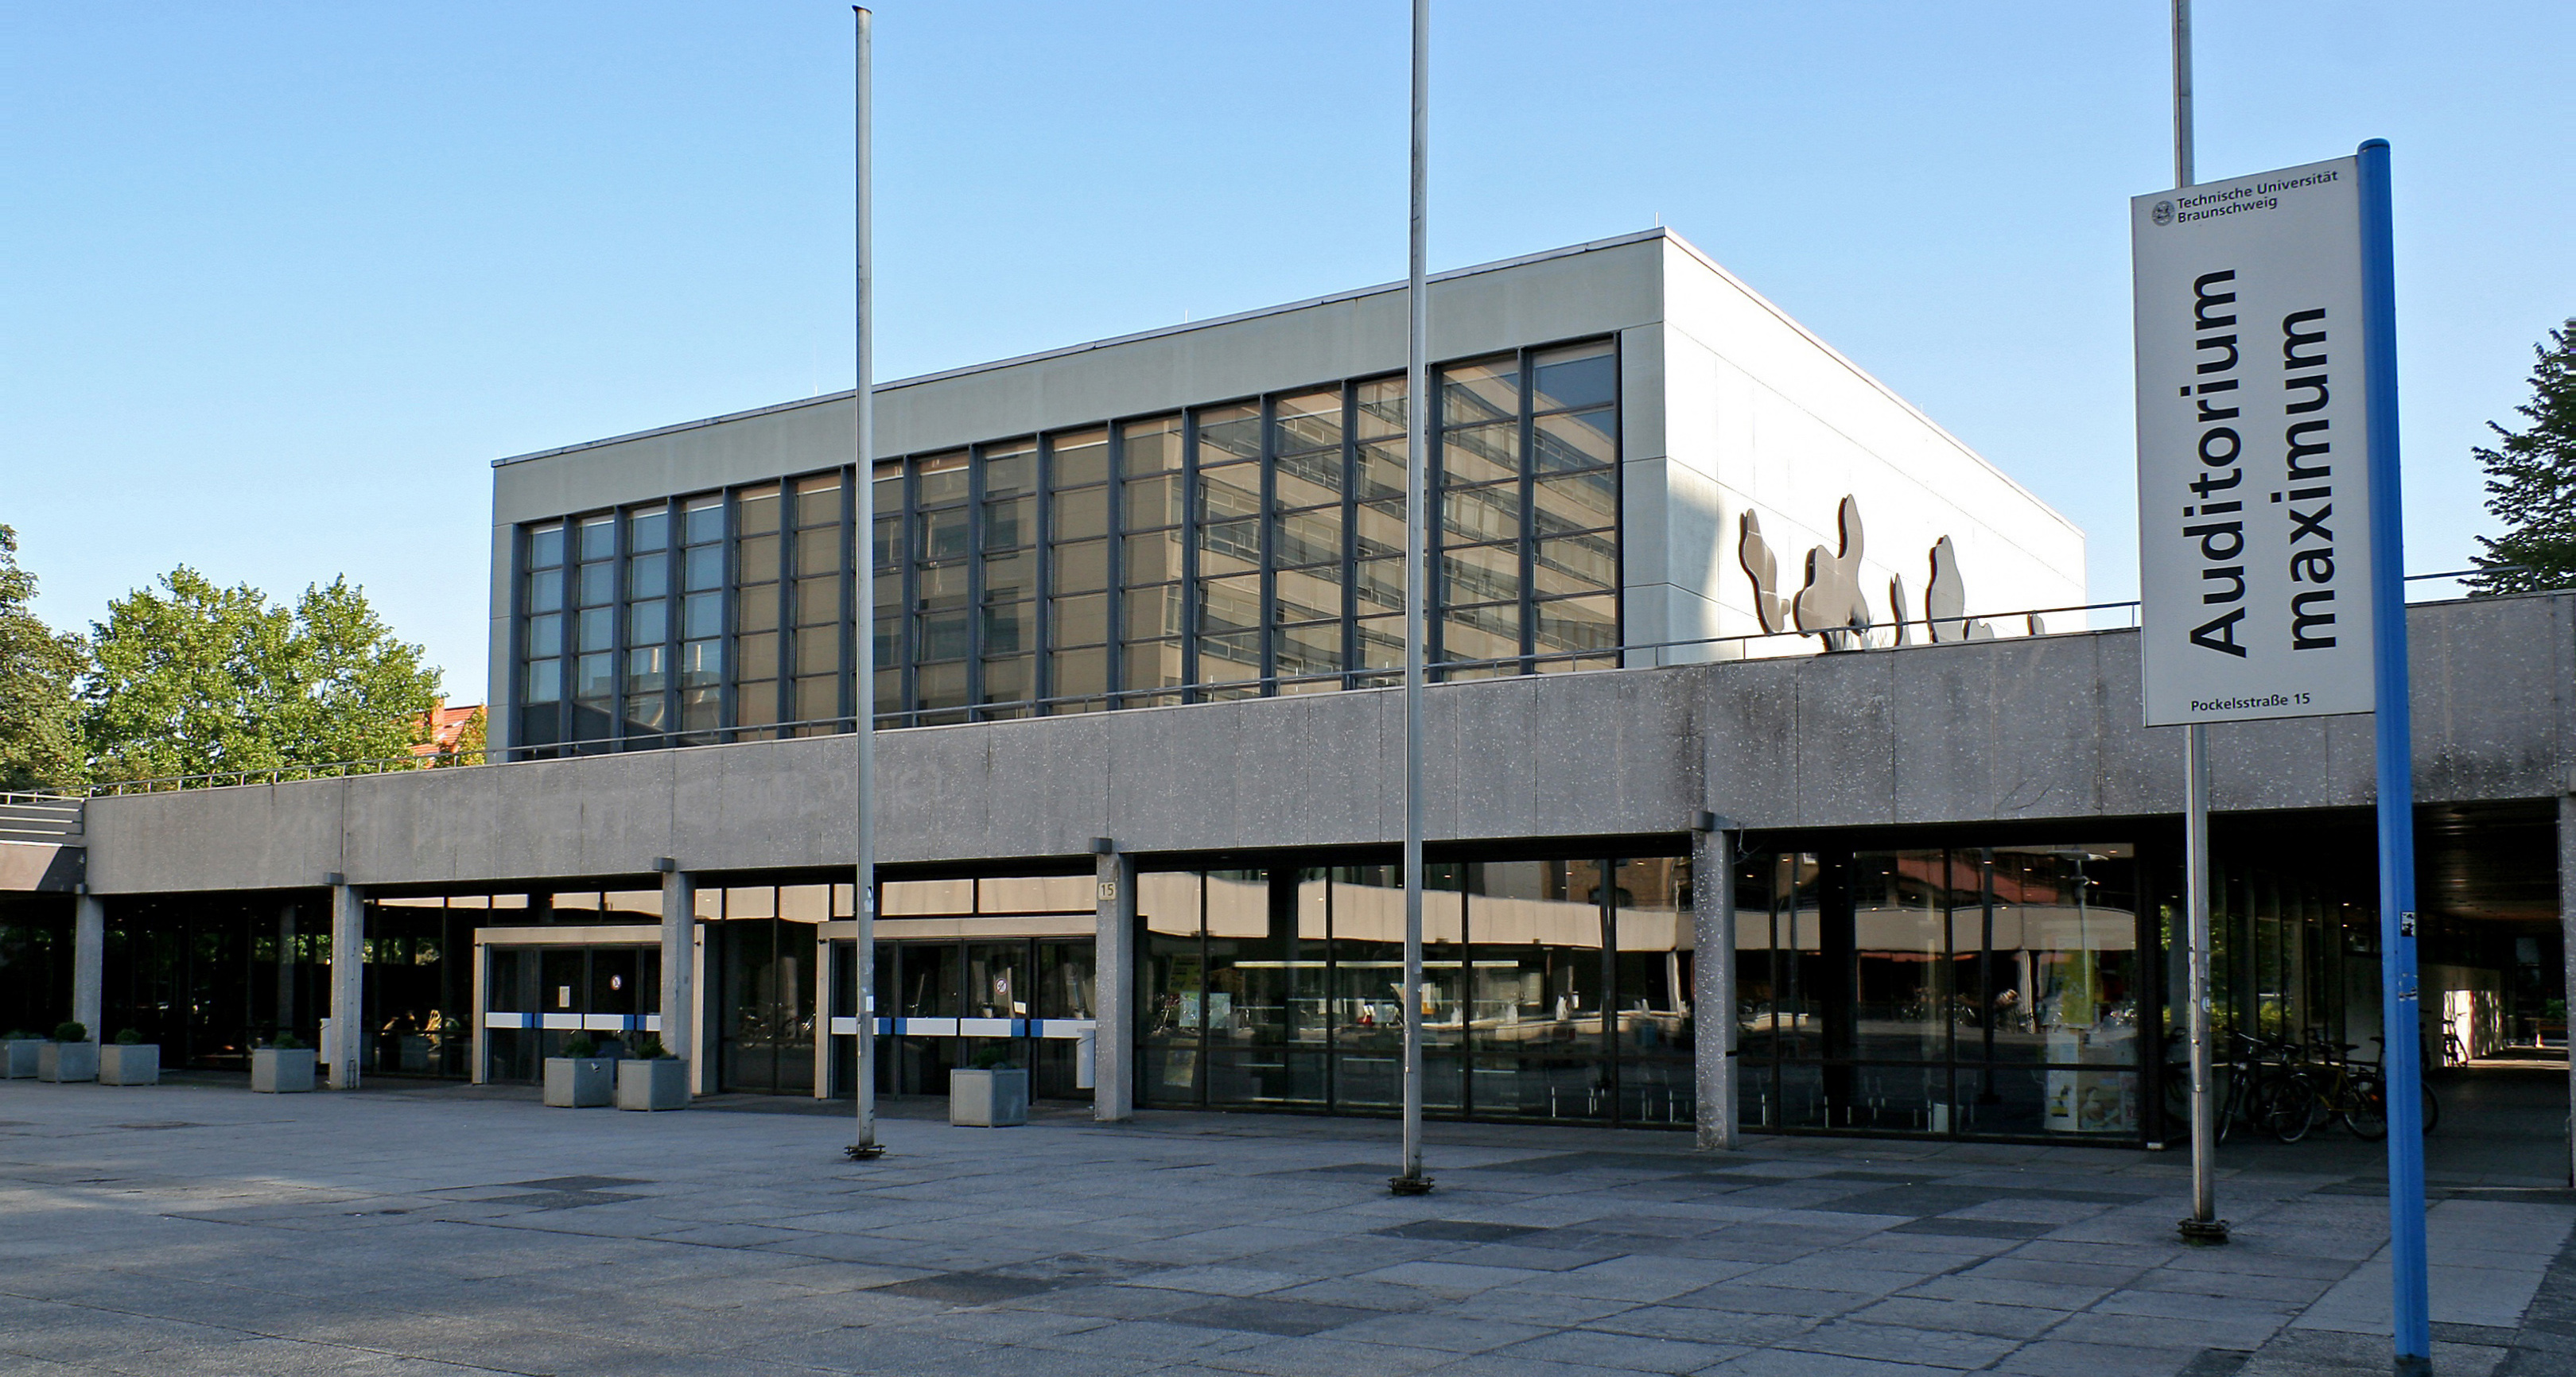
\includegraphics[width=\titlegraphicswidth]{titlepicture}}
\logo{
\includegraphics[height=\logoheight]{institut.jpg}}

\begin{document}

\begin{frame}[plain]
  \titlepage
\end{frame}

\begin{frame}{Inhaltsseite}
  \begin{itemize}
    \item Hier steht der Inhalt
    \item Hier nicht
    \item Weitere Informationen
  \end{itemize}
\end{frame}

\end{document}
\end{verbatim}

\begin{center}
  \fbox{\includegraphics[width=0.9\textwidth]{examples/titelseite.pdf}}

  \fbox{\includegraphics[width=0.9\textwidth]{examples/inhaltsseite.pdf}}
\end{center}
  % Kapitel: 'Präsentationen'


\chapter{Hintergrundlayout}

\begin{Declaration}
  \Macro{showtubslogo}\OParameter{Position}
\end{Declaration}

\begin{Declaration}
  \Macro{showlogo}\PParameter{Logo}
\end{Declaration}

\begin{Declaration}
  \Macro{showtopline}
\end{Declaration}

\begin{Declaration}
  \Macro{bgelement}\OParameter{Darstellung}\PParameter{Höhe}
\end{Declaration}

Erstellt ein Hintergrundelement im Gaußraster mit angegebener \PName{Höhe}.
Der Parameter \PName{Darstellung} kann die folgenden Einstellungen verarbeiten:

\begin{Declaration}
  \KOption{bgcolor}\PName{Farbe}\\
  \KOption{bgimage}\PName{Bild-Datei}\\
  \KOption{imagefit}\PName{Darstellungsoption}
\end{Declaration}

Mit \OptionValue{bgcolor}{Farbe} wird das Hintergrundelement mit der angegebenen
Farbe gefüllt.

Die Option \OptionValue{bgimage}{Bild-Datei} erlaubt dagegen die Darstellung
eines Hintergrundbildes im Element.
Da der Darstellungsbereich fest vorgegeben ist, muss das eingebundene Bild
in diesen Bereich eingepasst werden. Dies geschieht automatisch, die Art
der Einpassung lässt sich aber mit der Option \Option{imagefit} kontrollieren.
Sie erlaubt folgende Einstellungen:


\begin{desctable}
\entry{\PValue{cropped}}{%
  Automatisches Abschneiden. Dies ist die Standardeinstellung.
}
\entry{\PValue{cropx}}{%
  Abschnitt horizontal.
}
\entry{\PValue{cropy}}{%
  Abschnitt vertikal.
}
\entry{\PValue{scaled}}{%
  Horizontale \emph{und} vertikale Skalierung.
}
\end{desctable}


\chapter{Farben}\label{sec:tubscolors}
\Index{Farben|indexbf}

\newcommand{\classoptionitem}[1][ ]{
  \item[\mdseries{\ttfamily%
    \textbackslash usepackage%
    {[{\color{tuRed}#1}]}%
    \{tubslogo\}}]\hfill\\
}

Die Farbdefinitionen in \tubslatex werden vom Paket \newpackage{tubscolors}
zur Verfügung gestellt. Die folgende Beschreibung bezieht sich
auf den Funktionsumfang dieses Paketes.
Da das Paket aber in allen verfügbaren \tubslatex-Klassen fest eingebunden ist,
gelten die Erklärungen auch allgemein.

\newcommand{\rainbow}[2][\relax]{{\noindent\sffamily\footnotesize%
\ifx#1\relax\colorlet{fglbg}{black}\else\colorlet{fglbg}{#1}\fi
\colorbox{#2100}{\hbox to 0.188\textwidth{%
  \color{fglbg}\vphantom{Fg}#2{}100\hfill}}% 
\colorbox{#280}{\hbox to 0.188\textwidth{%
  \color{fglbg}\vphantom{Fg}#2{}80\hfill}}% 
\colorbox{#260}{\hbox to 0.188\textwidth{\vphantom{Fg}#2{}60\hfill}}% 
\colorbox{#240}{\hbox to 0.188\textwidth{\vphantom{Fg}#2{}40\hfill}}% 
\colorbox{#220}{\hbox to 0.188\textwidth{\vphantom{Fg}#2{}20\hfill}}\\% 
}}

\section{Verfügbare Farben}

Der Farbklang der TU-Braunschweig ist in eine Primär- und einen
Sekundärfarbbereich aufgeteilt.

Die Primärfarben bilden dabei Rot, Schwarz und Weiß, sowie in
20-Prozent-Schritten abgestufte Grautöne. Die Primärfarben dienen
vor allem zur Auszeichnung von Hintergrund, Textfarbe und dem TU-Logo.
Zur individuellen Gestaltung von Dokumenten ist der Sekundärfarbbereich
vorgesehen.

Die Sekundärfarben setzen sich aus 12 weiteren aufeinander abgestimmten
Farben zusammen, die 
in 4 Farbklänge (Gelb-Orange, Grün, Blau und Violett) mit je 3 Basisfarben
aufgeteilt sind.
Alle Sekundärfarben können in 20-Prozent-Schritten aufgehellt werden.

\subsection{Benennungsschema}
\Index{Farben!Benennungsschema}

Alle Farben tragen das Präfix \texttt{tubs} vor Ihrem Namen.
Der eigentliche Farbname setzt sich zusammen aus dem Namen
des Sekundärfarbklangs
(\texttt{Orange}, \texttt{Blue}, \texttt{Green}, \texttt{Violet}) 
und einer Farbvariante
(\texttt{Light}, \texttt{Medium}, \texttt{Dark})
gefolgt von der Prozentzahl ihrer Helligkeitsstufe
(\texttt{20}, \texttt{40}, \texttt{60}, \texttt{80}, \texttt{100}).

Die Farben können sowoh in Präfix-Notation
(\Color{tubs\textsf{<Variante>}\textsf{<Klang>}80})
als auch in Suffix-Notation (\Color{tubs\textmd{<Klang>}\textmd{<Variante>}80})
angegeben werden.

\begin{example}
  Die helle Variante des Blau in 60\%iger Helligkeit kann also
  über den Namen \Color{tubsBlueLight60} als auch
  \Color{tubsLightBlue60} gewählt werden.
\end{example}

Vereinfachte Varianten der Benennung gibt es unter anderem für die 100\%-Varianten.
Hier kann die Prozentzahl weggelassen werden.
\begin{important}
Die Primärfarbe \Color{tubsRed} ist \emph{nicht} identisch mit \Color{tubsRed100}
aus dem gelb-orange-Sekundärfarbbereich.
In diesem speziellen Fall handelt es sich um verschiedene Farben.
\end{important}
Auch für die \texttt{Medium}-Varianten ist kein Präfix/Suffix notwendig.
\begin{example}
  Die Medium-Variante des Grün in 100\%iger Helligkeit kann vereinfacht
  mit \Color{tubsGreen} bezeichnet werden.
\end{example}

Die drei Primärfarben rot, schwarz und weiß sind unter den Namen
\Color{tubsRed}, \Color{tubsBlack} und \Color{tubsWhite} verfügbar.

Im Folgenden werden die zu Verfügung stehenden Farben aufgelistet.
Die Standardnamen über die die einzelnen Farben angesprochen werden können,
sind in den Beispielfeldern angegeben.

\subsection{Primärfarben}
\Index{Primärfarben}
\Index{Farben!Primär-}

{\sffamily\footnotesize%
\colorbox{tubsRed}{\hbox to 0.188\textwidth{%
  \vphantom{Fg}tubsRed\hfill}}%
\colorbox{tubsBlack}{\hbox to 0.188\textwidth{%
  \color{white}\vphantom{Fg}tubsBlack\hfill}}%
\fcolorbox{tubsBlack}{tuWhite}{\hbox to 0.188\textwidth{%
  \vphantom{Fg}tubsWhite\hfill}}\\%
}

\rainbow[tuWhite]{tubsGray}

Zur Vereinfachung sind noch die Farben \Color{tubsGray} und
\Color{tubsLightGrey} definiert, die den Farben \Color{tubsGray60} und
\Color{tubsGray20} entsprechen.

Alle Graytöne sind darüber hinaus auch in britischer Schreibweise nutzbar
(\Color{tubsGrey}).


\pagebreak
\subsection{Sekundärfarben}
\Index{Sekundärfarben}
\Index{Farben!Sekundär-}

  tubsOrange\ldots\\
  \colorshow{Orange}{Light}
  \colorshow{Orange}{Medium}
  \colorshow{Orange}{Dark}\\[-1ex]
  tubsBlue\ldots\\
  \colorshow{Blue}{Light}
  \colorshow{Blue}{Medium}
  \colorshow{Blue}{Dark}\\[-1ex]
  tubsGreen\ldots\\
  \colorshow{Green}{Light}
  \colorshow{Green}{Medium}
  \colorshow{Green}{Dark}\\[-1ex]
  tubsViolet\ldots\\
  \colorshow{Violet}{Light}
  \colorshow{Violet}{Medium}
  \colorshow{Violet}{Dark}
%   \caption{Im CD definierte Farben und deren Benennung (Auszug)}


% \begin{example}
% In folgendem Beispiel wurde \lstinline{blau} als Farbklang ausgewählt:
% 
% tubsSecondary\ldots\\
% \colorshow{Secondary}{Light}
% \colorshow{Secondary}{Medium}
% \colorshow{Secondary}{Dark}\\[-1ex]
% \end{example}

\subsection{Farbmodelle}
\Index{Farbmodelle}

Die Farben sind für 3 Farbmodelle (\acrshort{RGB}, RGB beamer-optimiert, \acrshort{CMYK}) definiert.
Das gewünschte Farmodell kann durch Klassen- bzw. Paketoptionen gewählt werden.
Die einzelnen Klassen haben bereits das jeweils passende Farbmodell voreingestellt.

Zusätzlich kann eine Monochrom-Variante gewählt werden, die die Farbe
\Color{tusbRed} automatisch als Schwarz darstellt.


\clearpage
\section{Verwendung/Farbwahl}
\sloppy

% TODO: hier ist noch etwas Bedarf...

Die TU-Farben können nach dem oben erläuterten Schema abgerufen und verwendet
werden wie jede andere Farbe auch.

\paragraph{Haupt-Sekundärfarbklang}\label{sec:secondary}

Die Farben des aktuell gewählten Haupt-Sekundärfarbklangs können zusätzlich
über die Namen \Color{tuSecondaryLight},
\Color{tuSecondaryMedium}, \Color{tuSecondaryDark}, sowie die
entsprechenden Prozentualwert \Color{tuSecondaryLight20},
\Color{tuSecondaryLight40}, \ldots) angesprochen werden können.
Dies erlaubt eine flexible Verwendung der 4 Sekundärfarbklänge.

Die Wahl der Haupt-Sekundärfarbklangs erfolgt entweder über die weiter
unten beschriebenen Klassen-/Paketoptionen oder innerhalb des Dokumentes auch
mit dem Befehl \Macro{selectsecondary}.

\paragraph{Fettes Schwarz}\label{sec:richblack}
\Index{rich black|indexbf}
\Index{Schwarz!fettes|indexbf}

Bei der Verwendung des CMYK-Farbraums ist zu beachten,
dass das die Farbe Schwarz (\Color{tubsBlack})
der Mischung 0\%C, 0\%M, 0\%Y, 100\%K entspricht,
was in der Bildschirmdarstellung meist nur als sehr dunkles grau wahrgenommen wird.
Dies gilt somit auch für den Text im Dokument und ist normal.
Für Bildschirmdarstellung wird immer das RGB-Farbprofil empfohlen.

\begin{figure}[!ht]
\centering
{\selectcolormodel{cmyk}
\colorbox[cmyk]{0,0,0,1}{\parbox[t][2cm]{3cm}{\vfill\centering\sffamily\color{tubsWhite} tubsBlack\vfill}}%
\qquad
\colorbox[cmyk]{0.75,0.68,0.67,0.9}{\parbox[t][2cm]{3cm}{\vfill\centering\sffamily\color{tubsWhite} tubsRichBlack\vfill}}%
}
\caption{Vergleich der Farben \Color{tubsBlack} und \Color{tubsRichBlack} im CMYK-Farbraum}
\end{figure}


Im CMYK-Druck dagegen wird es mit der Key-Patrone gedruckt und daher korrekt
als Schwarz ausgegeben.
Sollte trotz dessen die Ausgabe aus dem Drucker zu hell erscheinen,
so kann dies entweder durch Verwendung der Klassen-/Paketoption \Option{richblack}
(siehe folgendes Kapitel) oder durch einen manuelle Anpassung der Farbe
\Color{tubsBlack} korrigiert werden, indem ein sogenanntes
\emph{Fettes Schwarz} (rich black) verwendet wird.
Dabei werden zusätzlich die CMY-Farben benutzt, um ein möglichst dunkles
Schwarz zu mischen. Die Standarddefinition der Option \Option{richblack}
entspricht dies  einer Mischung von 75\%C, 68\%M, 67\%Y, 90\%K.
Alternativ kann auch die definierte Farbe \Color{tubsRichBlack} verwendet werden.

Zu beachten ist jedoch, dass diese Farbe im Druck ggf. zu unsaubereren
Ergebnissen durch den übermäßigen Tinteneinsatz führen kann!
  
\begin{example}
  Manuelle Umdefinierung von \Color{tubsBlack}:\\
  \lstinline!\definecolor{tubsBlack}{CMYK}{0.5,0.5,0.5,1.0}!
\end{example}


\subsection{Paket-/Klassenoptionen und Befehle}
\Index{RGB}
\Index{RGB!Beamer}
\Index{CMYK}
\Index{monochrom}

\begin{Declaration}
  \Option{rgb}\\
  \Option{rgbbeamer}\\
  \Option{cmyk}\\[1ex]
  \Option{mono}
\end{Declaration}

Die Option \Option{rgb} bewirkt eine Darstellung der Farben im vordefinierten
RGB-Farbprofil.
Die Option \Option{rgbbeamer} lädt ein Beamer-optimierts RGB-Farbprofil.
Mit der Option \Option{cmyk} wird das CMYK-Farbprofil geladen.
Die Zusatz-Option \Option{mono} bewirkt eine Darstellung der Farbe
\Color{tubsRed} als \Color{tubsBlack} im aktuell gewählten Farbprofil.
Dies kann insbesondere für schwarz-weiß Kopiervorlagen in Verbindung
mit der schwarzen Siegelbandlogo-Variante sinnvoll sein.


\begin{Declaration}
  \Option{richblack}
\end{Declaration}

Definiert die Farbe \Color{tubsBlack} bei Verwendung des CMYK-Farbprofils
in ein sog. "`fettes Schwarz"' um. Siehe dazu auch Abschnitt~\ref{sec:richblack}.

\begin{Declaration}
  \Option{orange}\\
  \Option{green}\\
  \Option{blue}\\
  \Option{violet}
\end{Declaration}

Mit diesen Optionen kann der Standard-Sekundärfarbklang des Dokumentes gewählt
werden. Der jeweils geladene Sekundärfarbklang ergibt sich aus dem Namen
der Option.
Die Farben des Sekundärfarbklangs können wie in Abschnitt~\ref{sec:secondary}
beschrieben benutzt werden.

\begin{Declaration}
  \Macro{selectsecondary}\Parameter{Farbklang}
\end{Declaration}

Befehl zur Wahl des Haupt-Sekundärfarbklangs. Als Option für \PName{Farbklang}
sind die Werte \PValue{orange}, \PValue{green}, \PValue{blue} und \PValue{violet}
erlaubt.

\begin{Declaration}
  \Macro{tubscolorshow}\Parameter{Farbe}\Parameter{Variante}
\end{Declaration}

Zeigt farbige Boxen mit allen Helligkeitsstufen der angegebenen Farbklang-Variante.
\begin{example}
 Die Ausgabe von \lstinline!\tubscolorshow{Blue}{Light}! sieht beispielsweise
 wie folgt aus:\\
 \hspace*{-1cm}\tubscolorshow{Blue}{Light}
\end{example}

\fussy
  % Kapitel: 'Farben'

%Befehle für Glossar
\newglossaryentry{glos:siegelbandlogo}{%
  name=Siegelbandlogo,
  description={\tubslogo}
}
\newglossaryentry{glos:gaussraster}{%
  name={Gau\ss raster},
  description={Auf der gaußschen Summenformel basierende Unterteilung der Seite
    in Segmente. Benachbarte Segmente können beliebig zusammen gefasst werden}
}
\newglossaryentry{glos:cmyk}{%
  name={CMYK-Farbmodell},
  description={Das CMYK-Farbmodell ist ein subtraktives Farbmodell,
    das die technische Grundlage für den modernen Vierfarbdruck bildet.
    Die Abkürzung CMYK steht für die drei Farbbestandteile
    \emph{Cyan}, \emph{Magenta}, \emph{Yellow}
    und den Schwarzanteil \emph{Key} als Farbtiefe}
}
\newglossaryentry{glos:absenderbereich}{%
  name={Absenderbereich},
  description={Bereich zur Darstellung von Absendern}
}
\newglossaryentry{glos:kommunikationsbereich}{%
  name={Absenderbereich},
  description={Bereich zur Darstellung von Inhalten}
}
\newglossaryentry{glos:spaltenraster}{%
  name={Spaltenraster},
  description={Abhängig vom Format kann der Textbereich einer Seite in
    6, 4 oder 2 Grundspalten geteilt werden, welche alle die selbe Breite und
    den selben Abstand zueinander haben.
    Benachbarte Grundspalten können variabel zu einer Darstellungsspalte
    zusammengefasst werden}
}
\newglossaryentry{glos:bindekorrektur}{%
  name={Bindekorrektur},
  description={}
}
\newglossaryentry{glos:sekundaerfarbklang}{%
  name={Sekund\"arfarbklang},
  description={}
}

%Akronyme
\newacronym{CD}{CD}{Corporate Design}
\newacronym{CMYK}{CMYK}{Cyan, Magenta, Yellow, Key}


\end{document}
